\documentclass{beamer}
\usepackage{amsmath,amssymb,latexsym,array,fancyheadings,mathdots}
\usepackage{algorithm,algorithmic}
\usepackage{hyperref}
\usepackage{color}
\usepackage{tabularx}
\usepackage[all]{xy}
\usepackage{qtree}
\usepackage{gitinfo2}

%% RCS
%\usepackage{rcs}

%% Colors
\definecolor{darkgreen}{rgb}{0,.4,0}
\definecolor{darkred}{rgb}{.5,0,0}
\definecolor{darkmagenta}{rgb}{.5,0,.5}
\definecolor{orange}{rgb}{1,.5,0}
\definecolor{lightblue}{rgb}{0.122,0.016,0.855}
\definecolor{darkocre}{rgb}{0.471,0.298,0.008}

\usetheme{default}

%% New Theorems
\newtheorem{thm}{Theorem}
\newtheorem{exm}[thm]{Example}
\newtheorem{cor}[thm]{Corollary}
\newtheorem{propo}[thm]{Proposition}
\newtheorem{lem}[thm]{Lemma}
\newtheorem{clm}[thm]{Claim}
\newtheorem{exr}[thm]{Exercise}
\newtheorem{dfn}[thm]{Definition}

%% New commands
\newcommand{\classfont}{\mathsf}
\newcommand{\ATM}{\classfont{A}_{\mathrm{TM}}}
\newcommand{\MTF}{\mathrm{MTF}}
\newcommand{\OPT}{\mathrm{OPT}}
\newcommand{\ALG}{\mathrm{ALG}}
\newcommand{\ALGNAIVE}{\mathrm{ALG}_{\text{na{\"\i}ve}}}
\newcommand{\LRU}{\mathrm{LRU}}
\newcommand{\FIFO}{\mathrm{FIFO}}
\newcommand{\FWF}{\mathrm{FWF}}
\newcommand{\LFD}{\mathrm{LFD}}
\newcommand{\true}{\mathsf{T}}
\newcommand{\false}{\mathsf{F}}
\newcommand{\also}{\wedge}
\newcommand{\lra}{\leftrightarrow}
\newcommand{\tc}{\textcolor}
\newcommand{\df}[1]{\textcolor{red}{\em #1}}
\newcommand{\highlight}[1]{\textcolor{orange}{\em #1}}
\newcommand{\hl}[1]{\textcolor{blue}{\em #1}}
\newcommand{\amp}{\texttt{\&}}
\newcommand{\hsh}{\texttt{\#}}
\newcommand{\ra}{\rightarrow}
\newcommand{\longra}{\longrightarrow}
\newcommand{\Ra}{\Rightarrow}
\newcommand{\rab}{{\rightarrow_\beta}}
\newcommand{\srab}{{\rightarrow^*_\beta}}
\newcommand{\aeq}{{=_\alpha}}
\newcommand{\order}{\mathrm{order}}
\newcommand{\rem}{\mathrm{rem}}
\newcommand{\IP}{\mathbf{IP}}
\newcommand{\PSPACE}{\mathbf{PSPACE}}
\newcommand{\thevalue}{\text{value}}
\newcommand{\pol}[1]{\mathbf{#1}}
\newcommand{\enc}{\text{Enc}}
\newcommand{\xor}{\oplus}
\newcommand{\zo}{\{0,1\}}
\newcommand{\SOPT}{S_{\mathrm{opt}}}
\newcommand{\la}{\leftarrow}
\newcommand{\myurl}[1]{\textcolor{darkgreen}{\url{#1}}}
\newcommand{\myhref}[2]{\textcolor{darkgreen}{\href{#1}{#2}}}
\newcommand{\qaccept}{q_{\mathrm{accept}}}
\newcommand{\qreject}{q_{\mathrm{reject}}}
\newcommand{\opt}{\text{\sc Opt}}
\newcommand{\tr}{\mathrm{tr}}
\newcommand{\csanky}{p^{\textsc{csanky}}}
\newcommand{\berk}{p^{\textsc{berk}}}

%% Algorithms package customization
\renewcommand{\algorithmicrequire}{\textbf{Pre-condition:}} 
\renewcommand{\algorithmicensure}{\textbf{Post-condition:}} 
\algsetup{indent=3em}

\input{prooftree}

%% including/excluding pauses
\newcommand{\ifpause}{\iftrue} % for including pauses
%\newcommand{\ifpause}{\iffalse} % for excluding pauses

%% 2nd or 3rd edition
\newif\ifthird
\thirdtrue
%\thirdfalse

%disables usefoottemplate
\setbeamertemplate{navigation symbols}{}
%\setbeamertemplate{footline}% 
%{\strut\quad\tiny 
%\begin{minipage}{3cm}
%Cryptography - Michael Soltys
%\today\ {\tt v\RCSRevision}
%\end{minipage}\hfill
%\insertsection\
%- \insertframenumber/\inserttotalframenumber\quad\strut}

\newcommand{\mytitle}{Computational Foundations \\ Sections 9.1-9.2}
\newcommand{\mychpnr}{9}
%% Title page contents
\title{Intro to Analysis of Algorithms \\ \mytitle \\  Chapter \mychpnr}
\author{Michael Soltys}
\date{\textcolor{darkgreen}{\tiny\tt 
[ {\bf Git} Date:\gitAuthorDate\ 
Hash:\gitAbbrevHash\ 
Ed:\ifthird
3rd
\else
2nd
\fi]}}
\institute{CSU Channel Islands}

\setbeamertemplate{footline}{
  \colorbox{white}{\color{black}\tt
     \begin{tabularx}{0.97\textwidth}{XXX}
          IAA Chp \mychpnr\ - Michael Soltys \copyright & 
          \hfill\today\ (\gitAbbrevHash; \ifthird ed3\else ed2\fi)
					\hfill\phantom{.} & 
          \hfill\insertsection\ - \insertframenumber/\inserttotalframenumber \\
      \end{tabularx}}}

\begin{document}

\mode<presentation>
{
}

\parskip 8pt

\section{Introduction}

\begin{frame}
\titlepage
\end{frame}


\section{Introduction}

\section{Basics}

\begin{frame}
\begin{center}
\addtocounter{part}{1}
{\bf Sections 9.1 \&\ 9.2: \\ Alphabets, strings and languages}
\end{center}
\end{frame}

\begin{frame}
Since long ago ``markings'' have been used to store \&\ process information.
The following pictures are from the {\em Smithsonian Museum of Natural
History, Washington D.C.}
\begin{tabbing}
\begin{minipage}{6cm}
\raggedright
{\bf Engraved ocher plaque} \\
Blombos Cave, South Africa \\
77,000--75,000 years old
\end{minipage}
\=\begin{minipage}{6cm}
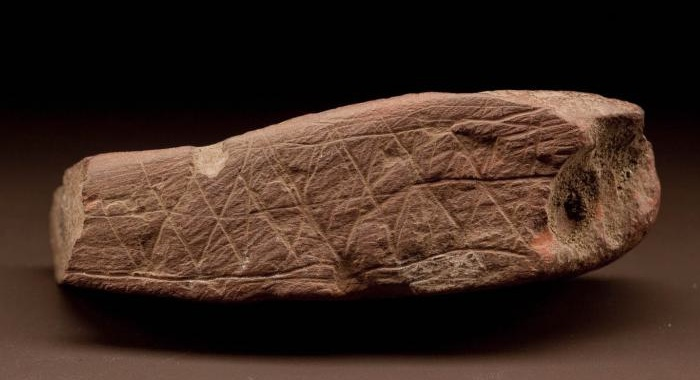
\includegraphics[width=2cm]{figures/ocher.jpg}
\hskip 2mm
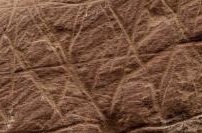
\includegraphics[width=3cm]{figures/ocher-zoom.jpg}
\end{minipage} \\[2mm]
\begin{minipage}{6cm}
\raggedright
{\bf Ishango bone} \\
Congo, 25,000--20,000 years old \\
leg bone from a baboon; 3~rows of tally marks,
to {\em add} or {\em multiply} ({\bf ?})
\end{minipage}
\>\begin{minipage}{5cm}
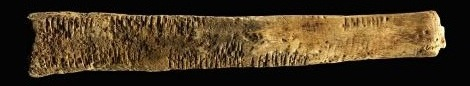
\includegraphics[width=5cm]{figures/ishango.jpg}
\end{minipage} \\[2mm]
\begin{minipage}{6cm}
\raggedright
{\bf Reindeer antler with tally marks} \\
La Madeleine, France \\
17,000--11,500 years old
\end{minipage}
\>\begin{minipage}{5cm}
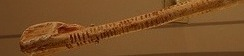
\includegraphics[width=5cm]{figures/antler.jpg}
\end{minipage}
\end{tabbing}
\end{frame}

\begin{frame}

About 8,000 years ago, humans were using symbols to represent words
and concepts.
True forms of writing developed over the next few thousand years. 

\begin{minipage}{5cm}
\raggedright
{\bf Cylinder seals} were rolled accross wet clay tablets to
produce raised designs \\[3mm]
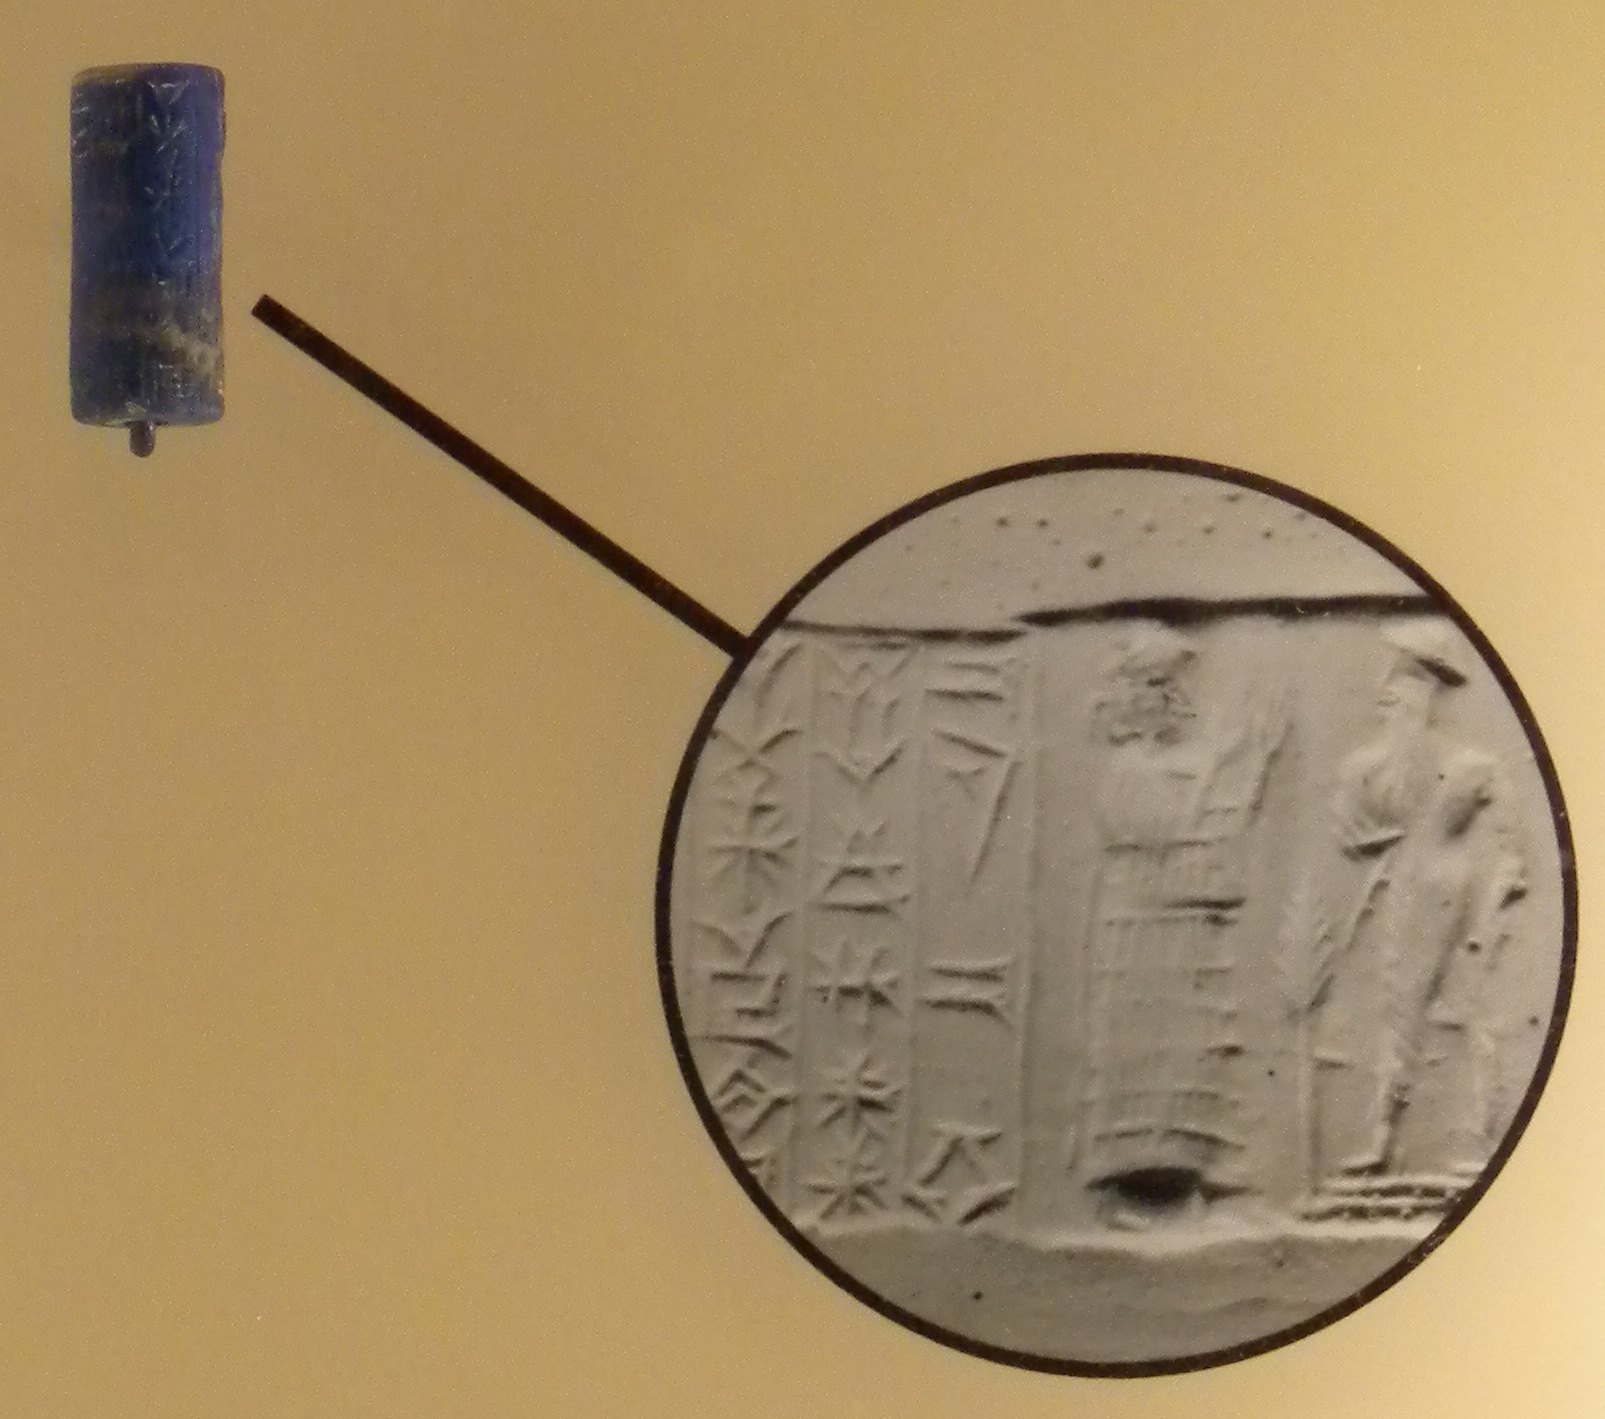
\includegraphics[width=4cm]{figures/cylinder.jpg} \\
cylinder seal in lapis lazuli,
Assyrian culture,
Babylon, Iraq,
4,100--3,600 years ago
\end{minipage}
\begin{minipage}{5.5cm}
\raggedright
{\bf Cuneiform symbols} stood for concepts and later for sounds and
syllables \\[3mm]
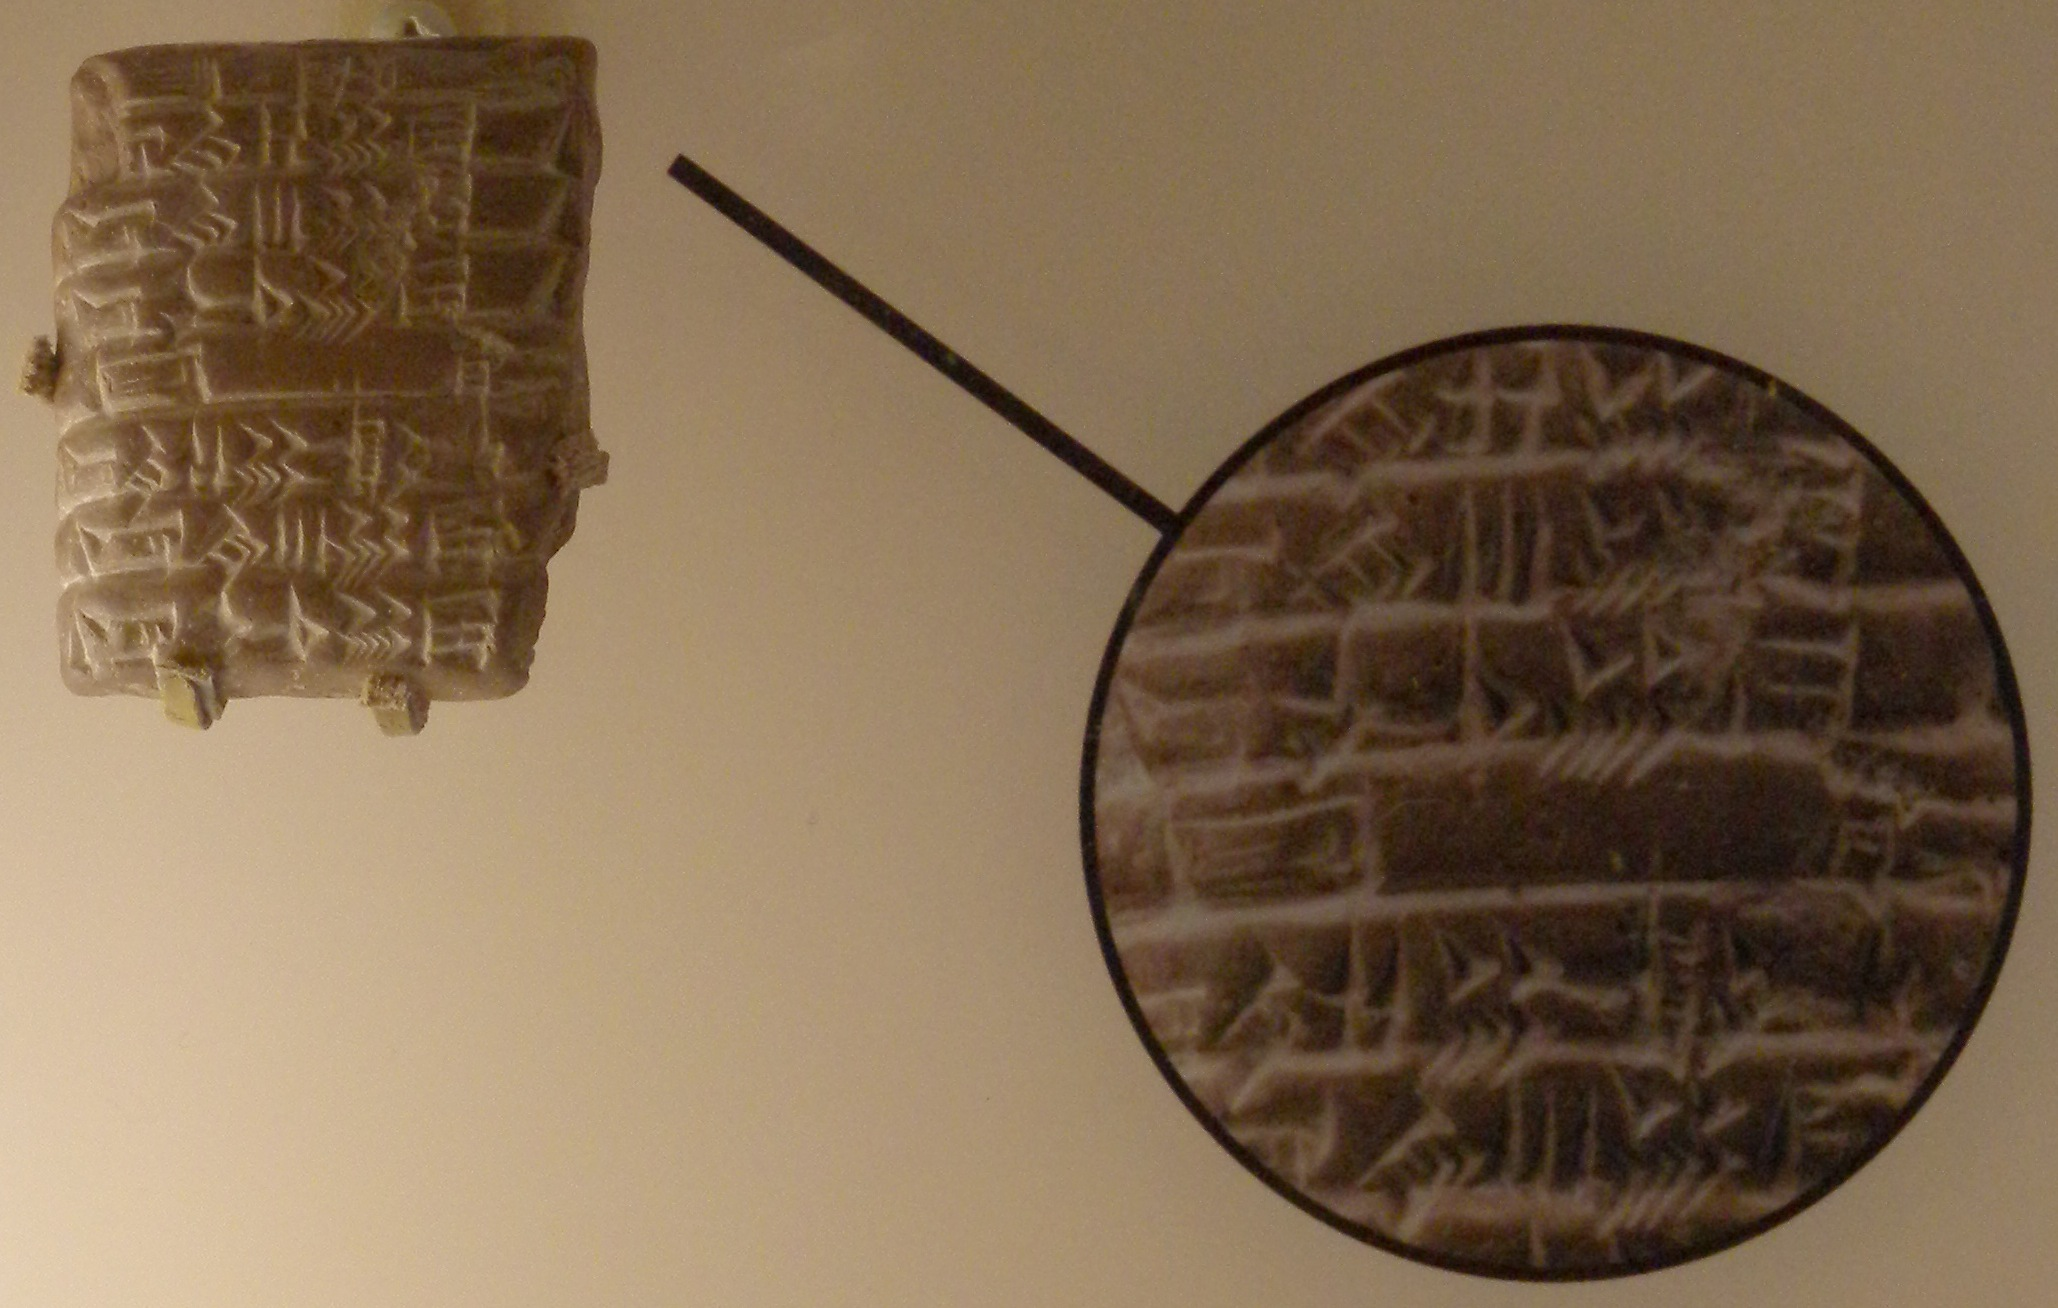
\includegraphics[width=5.5cm]{figures/cuneiform.jpg} \\
cuneiform clay tablet,
Chakma, Chalush, near Babylon, Iraq,
4,000--2,600 years ago
\end{minipage}
\end{frame}

\begin{frame}

\begin{center}
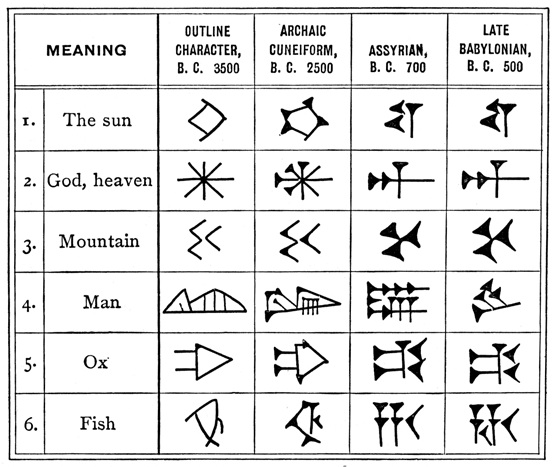
\includegraphics[width=8cm]{figures/cuneiform-symbols.jpg}
\end{center}
\end{frame}

\begin{frame}
An \df{alphabet} is a finite, non-empty set of
distinct symbols, denoted usually by $\Sigma$.

e.g., $\Sigma=\{0,1\}$ (binary alphabet) \\
$\Sigma=\{a,b,c,\ldots,z\}$ (lower-case letters alphabet)

A \df{string}, also called \df{word}, is a finite
ordered sequence of symbols chosen from some alphabet.

e.g., 010011101011

$|w|$ denotes the \df{length} of the string $w$.

e.g., $|010011101011|=12$

The \df{empty string}, $\varepsilon$,
$|\varepsilon|=0$, is in any $\Sigma$ by default.
\end{frame}

\begin{frame}
$\Sigma^k$ is the set of strings over $\Sigma$ of length {\em exactly}
$k$.  

e.g., If $\Sigma=\{0,1\}$, then 
\begin{align*}
\Sigma^0 &=\{\varepsilon\} \\
\Sigma^1 &=\Sigma \\
\Sigma^2 &=\{00,01,10,11\}, \text{ etc. } 
|\Sigma^k|?
\end{align*}

\df{Kleene's star}  $\Sigma^*$ is the set of all strings over
$\Sigma$.  

$\Sigma^*=\Sigma^0\cup
\underbrace{\Sigma^1\cup\Sigma^2\cup\Sigma^3\cup\ldots}_{=\Sigma^+}$

\df{Concatenation}  If $x,y$ are strings, and
$x=a_1a_2\ldots a_m$ \amp\ $y=b_1b_2\ldots b_n \Rightarrow$
$x\cdot y=\underbrace{xy}_{\text{\df{juxtaposition}}}
=a_1a_2\ldots a_mb_1b_2\ldots b_n$
\end{frame}

\begin{frame}
\begin{minipage}{5cm}
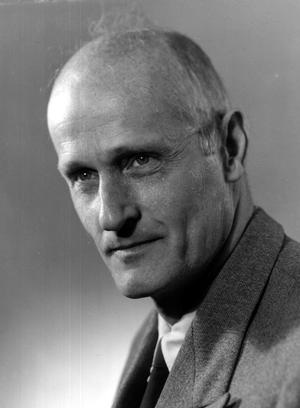
\includegraphics[width=4cm]{figures/StephenKleene.jpg}
\end{minipage}
\begin{minipage}{5cm}
\myhref{http://en.wikipedia.org/wiki/Stephen_Cole_Kleene}{Stephen Cole Kleene} \\
\end{minipage}
\end{frame}

\begin{frame}
A \df{language} $L$ is a collection of strings over some
alphabet $\Sigma$, i.e.,  $L\subseteq\Sigma^*$. E.g.,
\begin{equation}\label{eq:example}
L=\{\varepsilon,01,0011,000111,\ldots\}=\{0^n1^n|n\ge 0\}
\end{equation}

Note:

\begin{itemize}
\item  $w\varepsilon=\varepsilon w=w$.

\item $\{\varepsilon\}\neq\emptyset$; one is the language
consisting of the single string $\varepsilon$, and the other is the
empty language.

\end{itemize}
\end{frame}

\begin{frame}
Two fundamental questions:
\begin{itemize}
\item  How do we describe a language?  (\ref{eq:example}) is just an
{\em informal set-theoretic} description.

\item  Given a language $L\subseteq\Sigma^*$ and a string
$x\in\Sigma^*$, how do we check if $x\in L$?  E.g.,

$$
L=\{\underbrace{10}_2,\underbrace{11}_3,\underbrace{101}_5,
\underbrace{111}_7,\ldots\}\subseteq\{0,1\}^*
$$

$w\in L$ iff $w\in\{0,1\}^*$ encodes a prime number in standard binary
notation.

\item What is an algorithm?
\end{itemize}
\end{frame}

\end{document}
